%%%%%%%%%%%%%%%%%%%%%%%%%%%%%%%%%%%%%%%%%%%%%%%%%%%%%%%%%%%%%%%%%%%%%%%%%%%%%%%
%%
%%
%%
%%%%%%%%%%%%%%%%%%%%%%%%%%%%%%%%%%%%%%%%%%%%%%%%%%%%%%%%%%%%%%%%%%%%%%%%%%%%%%%


For Structure Rendering Use:
@Michal To Send example vesta files, font Avenir


Figures: Summary figure of found structures,
% ################################# Paragraph #################################
% AB2 Structures Ankit
- There are XYZ unique AB2 structures (or multiples, e.g. A2B4)
- Of those we found 697 unique AB2 prototypes (unique SG/Wyckoff combination) in OQMD/MP
- To generate our test set we substituted Ir for A and O for B, then isotropically expanded cell volume to constrain a minimum Ir-O distance of XYZ
- Next translated each of the 697 structures to be described by 271 features (invariant to isotropic expansion/compression), then reduced to 30 using PCA, described in methods XYZ
- To generate initial training data use existing DFT. Not enough on \ce{IrO_2}, so used OQMD to generate initial training data from nearest structures in phase space, described in Methods XYZ. Training set of 30 structures in SI XYZ.

% ################################# Paragraph #################################
% Iterative Training of Gaussian Process
- Trained Gaussian Process, rational quadratic kernel, variable length scales.
CV error of XYZ eV/atom, initial predictions in figure XYZ.
- Selected 10 structures with lowest prediction-uncertainty for DFT.
Structures were volume optimized, then fully relaxed, described in methods XYZ.
- Model retrained with the 10 DFT computed structures ONLY, 271 features->110 features applicable to \ce{IrO_2}->20 principle components for 99.9 percent variance.
CV error…
- Repeat until XYZ, final predictions shown in Fig XYZ

% #COMBAK FIGURE HERE
% Figure 2:  IrO2 initial and final predictions and uncertainties

% ################################# Paragraph #################################
% IrO2 Structure Analysis
- Describe relevant features
  - Physical intuition?
- Describe convex hull plot (energy vs. Ir-O distance), computed amorphous phase to define synthesizability
- While only 2 \ce{IrO_2} in MP/OQMD, we can compare our structures to other computed \ce{IrO_2} not in open databases.

% TEMP #COMBAK Remove dummy citation after real ones start coming in
This is a citation example \cite{dummy9999}.
Without it I think stuff breaks.


% | - Figure | IrO2 Convergence Plot
\begin{figure}
\centering
\makebox[\textwidth][c]{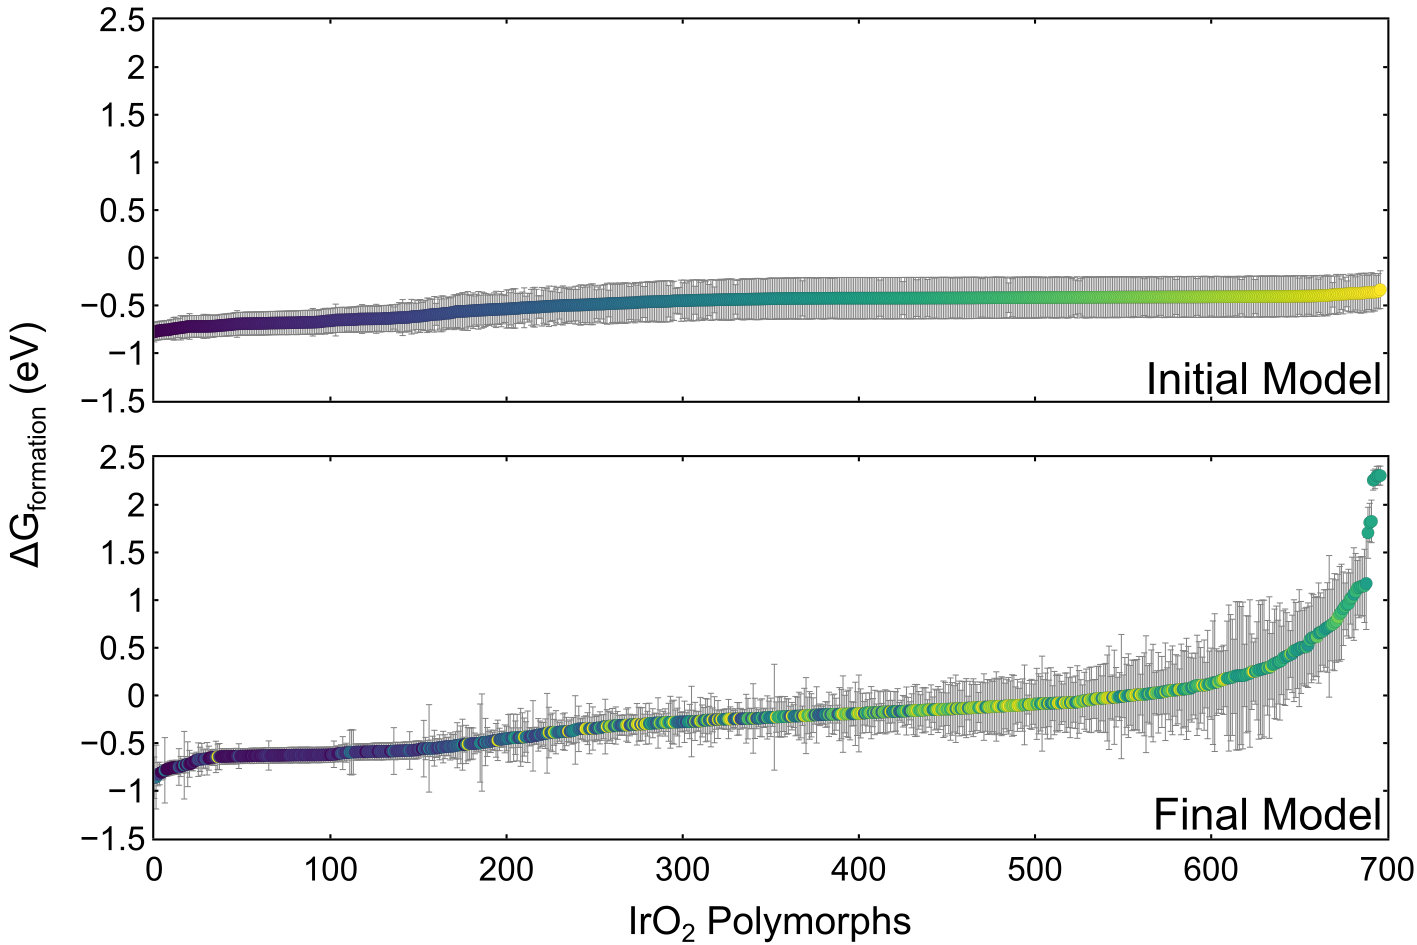
\includegraphics
  {02_figures/ml_convergence_plots/00_master__iro2-ml-conv_v1__200dpi__0__outplot.png}
  % {02_figures/ml_convergence_plots/iro2_ml_conv.png}
  }
\caption{\label{fig:convergence_plot_iro2_0}
  TEMP.
  }
\end{figure}
% __|
